% Figure: two audio representations. A log-mel spectrogram is an image (frame x mel band) that can be cut into patches or read frame by frame; a neural codec turns each latent step into S codes, each RVQ level quantizing what the previous levels left over.
% Design width ~168mm, height ~64mm.
\documentclass[border=0pt]{standalone}
\usepackage{amsmath,amssymb}
% Shared visual language for the figures of the book.
% Every figure in this directory loads this file so the chapter reads as one system.
% NOTE: no blank lines are allowed inside \tikzset{...} (a blank line emits \par
% and breaks key scanning).
\NeedsTeXFormat{LaTeX2e}
\ProvidesPackage{figstyle}[2026/10/21 Figure style for Free Energy to LLMs]

\RequirePackage{tikz}
\usetikzlibrary{arrows.meta,positioning,calc,fit,shapes.geometric,shapes.misc,%
  backgrounds,matrix,decorations.pathreplacing,decorations.markings,patterns.meta}

% ---------------------------------------------------------------- palette
% Same values as book/preamble/style.tex, prefixed with F.
\definecolor{FNavy}{HTML}{14324A}
\definecolor{FTeal}{HTML}{0E7490}
\definecolor{FSky}{HTML}{E7F5F8}
\definecolor{FOrange}{HTML}{D97706}
\definecolor{FAmber}{HTML}{FFF3D6}
\definecolor{FInk}{HTML}{1F2937}
\definecolor{FSlate}{HTML}{64748B}
\definecolor{FMist}{HTML}{F5F7FA}
\definecolor{FRose}{HTML}{9F1239}
\definecolor{FRoseMist}{HTML}{FFF1F2}

% ---------------------------------------------------------------- semantics
% Teal   = probability / model / data object
% Orange = training objective, cost, or the quantity moved through the system
% Navy   = neutral structure
% Slate  = secondary label or metadata
% Rose   = failure mode, hazard, masked-out region
\tikzset{
  % Lay figures out in millimetres.  A figure designed 168mm wide is included at
  % \textwidth, so its fonts appear at exactly the size written here.
  every picture/.style={x=1mm,y=1mm,font=\small,line cap=round,line join=round},
  % ---- block styles
  nbase/.style={draw,rounded corners=1.2pt,align=center,inner sep=2.4pt,%
    minimum height=7mm,text=FInk},
  nteal/.style={nbase,draw=FTeal,fill=FSky},
  norange/.style={nbase,draw=FOrange,fill=FAmber},
  nnavy/.style={nbase,draw=FNavy,fill=white},
  nsoft/.style={nbase,draw=FSlate!55,fill=FMist},
  nrose/.style={nbase,draw=FRose,fill=FRoseMist},
  ghost/.style={draw=none,fill=none,align=center,inner sep=1pt},
  plain/.style={draw=none,fill=none,align=center,inner sep=0pt},
  % ---- arrows
  ar/.style={-{Latex[length=1.7mm,width=1.35mm]},draw=FSlate,line width=0.75pt},
  ard/.style={ar,dashed},
  arteal/.style={ar,draw=FTeal},
  arorange/.style={ar,draw=FOrange},
  arrose/.style={ar,draw=FRose},
  thickar/.style={ar,line width=1.2pt},
  % ---- text roles
  ftitle/.style={font=\large\bfseries,text=FNavy,align=center},
  ptitle/.style={font=\small\bfseries,text=FNavy,align=center},
  ptitleo/.style={font=\small\bfseries,text=FOrange,align=center},
  lbl/.style={font=\scriptsize,text=FSlate,align=center,inner sep=1pt},
  lblt/.style={lbl,text=FTeal},
  lblo/.style={lbl,text=FOrange},
  lbln/.style={lbl,text=FNavy},
  lblr/.style={lbl,text=FRose},
  sub/.style={font=\scriptsize,text=FSlate!90,align=center,inner sep=1pt},
  monob/.style={font=\ttfamily\scriptsize,text=FInk,inner sep=1pt},
  mathb/.style={font=\small,text=FInk,inner sep=1pt},
  eqn/.style={font=\scriptsize,inner sep=1.5pt,text=FInk},
  % ---- decorations
  brace/.style={decorate,decoration={brace,amplitude=2.4pt},draw=FSlate,%
    line width=0.6pt},
  bracet/.style={brace,draw=FTeal},
  braceo/.style={brace,draw=FOrange},
  axis/.style={draw=FSlate!55,line width=0.6pt},
  guide/.style={draw=FSlate!45,line width=0.5pt,dashed},
  halolabel/.style={font=\scriptsize,text=FInk,fill=white,fill opacity=0.85,%
    text opacity=1,inner sep=1.4pt,align=center},
}

% Figure title above the drawing, anchored at the figure's top-left.
\newcommand{\figtitle}[2][0]{%
  \node[ftitle,anchor=north west,outer sep=0pt] at (#1,0) {#2};}

% Rounded panel behind a subgroup of nodes.
\newcommand{\figpanel}[3][]{%
  \node[draw=FSlate!35,fill=#3,rounded corners=2pt,inner sep=2.6mm,#1] {#2};}

\endinput

\begin{document}
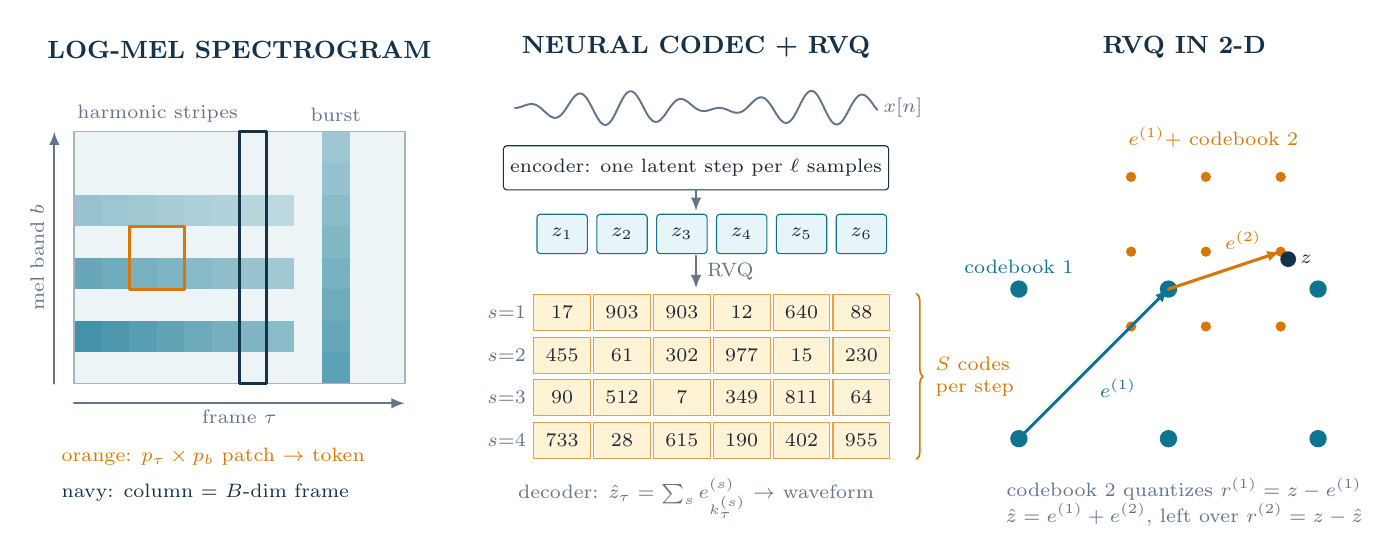
\begin{tikzpicture}
% ------------------------------------------------------- A: log-mel spectrogram
\node[ptitle,anchor=south] at (27,58) {LOG-MEL SPECTROGRAM};
\foreach \c in {0,...,11}{%
  \foreach \r in {0,...,7}{%
    \pgfmathsetmacro{\v}{%
      (\c<8)*((\r==1)*70+(\r==3)*55+(\r==5)*35)*(1-0.06*\c)%
      +(\c==9)*(60-4*\r)+8}%
    \fill[FTeal!\v!white] ({6+3.5*\c},{18+4*\r}) rectangle ++(3.5,4);%
  }%
}
\draw[axis] (6,18) rectangle (48,50);
\draw[FOrange,line width=1.1pt] (13,30) rectangle ++(7,8);
\draw[FNavy,line width=1.1pt] (27,18) rectangle ++(3.5,32);
\draw[ar] (6,15.5)--(48,15.5);
\node[lbl,anchor=north] at (27,15) {frame $\tau$};
\draw[ar] (3.5,18)--(3.5,50);
\node[lbl,rotate=90,anchor=south] at (2.6,34) {mel band $b$};
\node[lbl,anchor=south west] at (6,50.8) {harmonic stripes};
\node[lbl,anchor=south] at (39.25,50.8) {burst};
\node[lblo,anchor=north west,align=left] at (4,10.2) {orange: $p_\tau\times p_b$ patch $\to$ token};
\node[lbln,anchor=north west,align=left] at (4,5.6) {navy: column $=$ $B$-dim frame};
% ------------------------------------------------------- B: codec + RVQ grid
\node[ptitle,anchor=south] at (85,58) {NEURAL CODEC + RVQ};
\draw[FSlate,line width=0.7pt,domain=0:46,samples=140,smooth]
  plot ({62+\x},{53+2.2*sin(\x*55)*sin(\x*7)});
\node[lbl,anchor=west] at (108.4,53) {$x[n]$};
\node[nnavy,minimum width=46mm,minimum height=5.6mm,font=\scriptsize] (enc) at (85,45.4)
  {encoder: one latent step per $\ell$ samples};
\foreach \c in {0,...,5}{%
  \node[nteal,minimum width=6.4mm,minimum height=5mm,inner sep=0pt,font=\scriptsize]
    (z\c) at ({68+7.6*\c},37) {$z_{\the\numexpr\c+1\relax}$};%
}
\draw[ar] (enc.south)--++(0,-2.6);
\def\codes{{{17,903,903,12,640,88},{455,61,302,977,15,230},{90,512,7,349,811,64},{733,28,615,190,402,955}}}
\foreach \r in {0,...,3}{%
  \foreach \c in {0,...,5}{%
    \pgfmathsetmacro{\k}{\codes[\r][\c]}%
    \node[draw=FOrange!70,fill=FAmber,minimum width=7.2mm,minimum height=4.6mm,inner sep=0pt,font=\scriptsize\ttfamily,text=FInk]
      at ({68+7.6*\c},{27-5.4*\r}) {\pgfmathprintnumber[int detect]{\k}};%
  }%
}
\draw[ar] (85,34.2)--(85,30.1);
\node[lbl,anchor=west] at (86,32.2) {RVQ};
\foreach \r in {0,...,3}{%
  \node[lbl,anchor=east] at (63.8,{27-5.4*\r}) {$s{=}\the\numexpr\r+1\relax$};%
}
\draw[braceo] (113,29.4)--(113,8.4);
\node[lblo,anchor=west,align=left] at (115,18.9) {$S$ codes\\per step};
\node[lbl,anchor=north,align=center] at (85,6.4)
  {decoder: $\hat z_\tau=\sum_s e^{(s)}_{k^{(s)}_\tau}\to$ waveform};
% ------------------------------------------------------- C: RVQ in 2-D
\node[ptitle,anchor=south] at (147,58) {RVQ IN 2-D};
\def\ox{126}\def\oy{11}\def\u{19}
\foreach \i in {0,1,2}{%
  \foreach \j in {0,1}{%
    \fill[FTeal] ({\ox+\u*\i},{\oy+\u*\j}) circle (1.1);%
  }%
}
\foreach \a in {-0.25,0.25,0.75}{%
  \foreach \b in {-0.25,0.25,0.75}{%
    \fill[FOrange] ({\ox+\u*(1+\a)},{\oy+\u*(1+\b)}) circle (0.65);%
  }%
}
\draw[arteal,line width=1.1pt] (\ox,\oy)--({\ox+\u},{\oy+\u});
\draw[arorange,line width=1.1pt] ({\ox+\u},{\oy+\u})--({\ox+\u*1.75},{\oy+\u*1.25});
\fill[FNavy] ({\ox+\u*1.8},{\oy+\u*1.2}) circle (1.0);
\node[lbln,anchor=west] at ({\ox+\u*1.86},{\oy+\u*1.2}) {$z$};
\node[lblt,anchor=north west,align=left] at ({\ox+\u*0.52},{\oy+\u*0.42}) {$e^{(1)}$};
\node[lblo,anchor=south] at ({\ox+\u*1.3},{\oy+\u*1.92}) {$e^{(1)}+$ codebook 2};
\node[lblo,anchor=south] at ({\ox+\u*1.5},{\oy+\u*1.24}) {$e^{(2)}$};
\node[lblt,anchor=south] at ({\ox},{\oy+\u*1.08}) {codebook 1};
\node[lbl,anchor=north,align=center] at (147,6.4)
  {codebook 2 quantizes $r^{(1)}=z-e^{(1)}$\\$\hat z=e^{(1)}+e^{(2)}$, left over $r^{(2)}=z-\hat z$};
\end{tikzpicture}
\end{document}
